\documentclass[class=book, crop=false, oneside, 12pt]{standalone}
\usepackage{standalone}
\usepackage{amsmath}
\usepackage{../../style}
\graphicspath{{./assets/images/}}

\begin{document}

\chapter{Gravitazione}

\section{La forza gravitazionale}

\subsection{Introduzione}

Per parlare della forza gravitazionale è necessario richiamare alcune basi riguardanti il moto dei pianeti dell'era pre-Newtoniana.\newline
Verso il 1500 era stata avanzata da Copernico l'ipotesi eliocentrica: il Sole, e non la Terra, era il corpo celeste attorno al quale si svolgeva il moto dei pianeti.\newline
Dopo questa affermazione furono eseguite misure precise che Keplero utilizz\`o nel formulare le sue tre leggi.
Queste leggi ci danno una descrizione cinematica del moto dei pianeti.

\subsection{Leggi di Keplero}
\subsubsection{Prima legge}

I pianeti percorrono orbite ellittiche intorno al Sole che occupa uno dei fuochi dell'ellisse. 

\subsubsection{Seconda legge}

La velocità areale con cui il raggio vettore che unisce il Sole ad un pianeta descrive l'orbita è costante. 

\begin{figure}[h]
    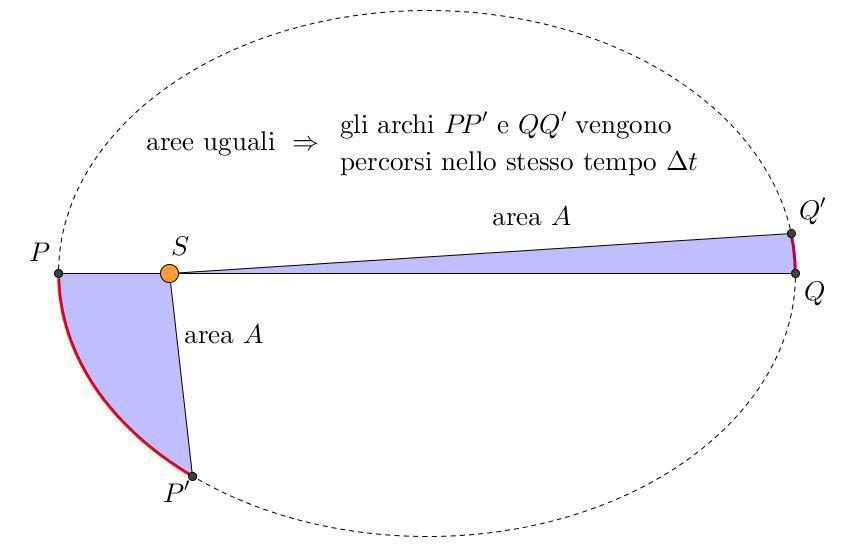
\includegraphics[scale=0.5]{keplero2}
    \centering
    \caption{}
\end{figure}

\subsubsection{Terza legge}

Il quadrato del periodo di rivoluzione di ogni pianeta è proporzionale al cubo del semiasse maggiore dell'ellisse: $T^2 = k r^3$

\subsection{Il ragionamento di Newton}

Le orbite dei pianeti, pur essendo certamente ellittiche, sono molto prossime a circonferenze; assumiamo che siano circolari.\newline
Se questo è vero e se la velocità areale è costante, il moto di un pianeta è circolare uniforme.
La forza che agisce sul pianeta, permettendogli di percorrere una traiettoria circolare  con velocità costante, deve essere esclusivamente centripeta:
\begin{equation}
    F = M \omega^2 r = m \left(\frac{2 \pi}{T}\right)^2 r
\end{equation}
con \(T\) il periodo di rivoluzione, \(m\) la massa e \(r\) il raggio dell'orbita del pianeta. 

Utilizziamo ora la terza legge di Keplero $T^2 = k r^3$, confondendo il raggio della circonferenza con il semiasse maggiore dell'ellisse (vista l'assunzione iniziale), così che la forza diviene
\begin{equation*}
    F = \frac{4 \pi^2}{k} \frac{m}{r^2}
\end{equation*}
Ottengo che la forza esercitata dal Sole sui pianeti, che incurva la loro orbita, è inversamente proporzionale al quadrato della distanza dal Sole.

Considerando il sottosistema Sole-Terra, la forza esercitata sulla Terra può quindi essere scritta:
\begin{equation*}
    F_{S,T} = \frac{4 \pi^2}{k_T} \frac{m_T}{r^2}
\end{equation*}
la forza esercitata dalla Terra sul Sole ha l'espressione:
\begin{equation*}
    F_{S,T} = \frac{4 \pi^2}{k_S} \frac{m_S}{r^2}
\end{equation*}
esse sono uguali in modulo per il terzo principio della dinamica.
Ottengo che \(m_t k_s = m_s k_t\).
Definendo la costante di gravitazione
\begin{equation}
    \gamma = \frac{4 \pi^2}{m_t k_s} = \frac{4 \pi^2}{m_s k_t}
\end{equation}
abbiamo il modulo della forza Sole-Terra
\begin{equation}
    F = \gamma \frac{m_s m_t}{r^2}
\end{equation}

\subsection{Legge di gravitazione universale}

La formula ottenuta è molto semplice ed è simmetrica nei due corpi; 
Newton ipotizzò che si trattasse di una formula universale ed enunciò la seguente legge di gravitazione universale: \newline
\emph{date due masse qualsiasi, di dimensioni trascurabili rispetto alla distanza mutua, tra di esse agisce una forza attrattiva diretta lungo la retta congiungente le due masse, il cui modulo dipende direttamente dal prodotto delle masse e inversamente dal quadrato della distanza.}\newline
La costante di proporzionalità \(\gamma\) è una costante universale, che non dipende dai valori delle masse e dalla geometria del sistema, ma è caratteristica dell'interazione gravitazionale.

In termini vettoriali ottengo che l'espressione della forza gravitazionale che la massa \(m_1\) esercita sulla massa \(m_2\) è:
\begin{equation}
    \overrightarrow{F_{1,2}} = - \gamma \frac{m_1 m_2}{r^2} \overrightarrow{u_{1,2}}
\end{equation}

Questa formula è valida se si ammette che un corpo a simmetria sferica eserciti una forza come se la massa fosse tutta concentrata nel suo centro.
So anche poi che \(F = mg\) per cui:
\begin{equation}
    g = \gamma \frac{m_T}{R^2}
\end{equation}
però Newton non sapeva n\'e \(m_T\) n\'e \(\gamma\) quindi fece riferimento al sistema Terra-Luna.
\begin{equation}
    F_{T,L} = \gamma \frac{m_T m_L}{r_L^2} = m_L \omega_L^2 r_L \Leftrightarrow \gamma m_T = \omega_L^2 r_L^3 \Leftrightarrow \gamma m_T = g r_L^2
\end{equation}
e dunque dal periodo di rivoluzione della Luna attorno alla Terra e dalla distanza Terra-Luna è possibile determinare \(g\).

I valori più attuali delle costanti sono:
\begin{equation*}
    \gamma = 6.67 \cdot 10^{-11} \udm{\frac{m^3}{kg s^2}} \ , \ m_T = 5.98 \cdot 10^{24} \udm{kg} .
\end{equation*}

A differenza delle forza che abbiamo visto precedentemente le interazioni fondamentali conosciute sono forze a distanza, che differiscono però nel raggio di azione (oltre che per altre proprietà): 
la forza gravitazionale e la forza tra cariche elettriche hanno la stessa dipendenza dalla distanza $\frac{1}{r^2}$ e si dice che il loro \emph{raggio di azione è infinito}.

\section{Massa inerziale e massa gravitazionale}

La \emph{legge di gravitazione universale} esprime un particolare tipo di interazione esistente in natura il cui valore numerico dipende da \(\gamma\), che è tipica dell'interazione, dalla geometria del sistema e da una caratteristica dei corpi che partecipano all'interazione, che abbiamo indicato con \(m\) e chiamiamo massa gravitazionale. 
A priori non c'è nessuna ragione logica per cui la massa gravitazionale, legata a una particolare interazione, debba essere eguale alla massa inerziale che compare nella legge di Newton, la massa inerziale.

Sperimentalmente, in uno stesso luogo \(g\) è indipendente dai corpi, quindi per qualsiasi corpo il rapporto $\frac{m_G}{m_I}$ è pari a una costante, indipendente dal corpo: 
le due masse \(m_I\) e \(m_G\) sono per lo meno proporzionali.
Poiché non c'è un modo diretto per misurare il rapporto $\frac{m_G}{m_I}$ l'ipotesi più semplice è supporre $\frac{m_G}{m_I}$, anche se il fatto che questi due valori siano uguali non ha spiegazione teorica.


\end{document}